 
This work on using a Gaussian Process for cosmic shear analysis 
was first discussed as a possibility in  \citep{Schneider2014}  and 
forms the basis of the analyses that I helped perform 
in Schneider et al. (in prep.). 

\section{Introduction} 

% why study cosmic shear 
A cornerstone of cosmology is found on the 
observation of the highly Gaussian temperature fluctuations in the cosmic microwave 
background (CMB). It is an ancient light emitted from the hot, primordial matter 
distribution in the early universe. 
% The high degree of Gaussianity in the CMB is a result of the spatial properties of the
% primordial density perturbations. 
% A number of inflation models can explain how these
% nearly Gaussian fluctuations could arise from quantum perturbations in the 
% early universe. 
We know how these primordial matter perturbations could grow 
through linear transfer over time to form a large-scale ($> 10 h^{-1} Mpc$) 
dark matter (DM) density field that is consistent with present
day observables. The large-scale dark matter distribution  
 encodes valuable information for constraining cosmological
parameters. Many gravitational lensing analyses of the large-scale DM density 
field, such as from
the Canadian-French-Hawaiian Telescope Lens survey (CFHTLens;
\citealt{Kilbinger2013}), the Deep Lens Survey
(DLS; \citealt{Jee2013a}, \citealt{Wittman2002}), the Dark Energy Survey 
(DES; \citealt{Abbott2016}) and others, 
have already given competitive cosmological constraints for 
 the matter density ($\Omega_m$) and the fluctuation amplitude 
of the matter density ($\sigma_8$) on a particular characteristic scale (8
$h^{-1} Mpc$). 
% The observable, the subtle distortion signals of galaxy shapes 
% that is induced by the gravity of intervening DM
% between far away galaxies and the observers, is also known as cosmic shear.  

% how complicated is cosmic shear inference 
% have already demonstrated the constraining power  
% constraints.
% This has sparked interests to
% come up with a comprehensive (statistical) framework to address the effects
% from systematics.

% As first discussed in chapter 1, the presence of DM could distort background
% galaxy shapes through gravitational lensing.
The analysis of the gravitational lensing signal from the DM density field, 
however, is far from trivial. 
In Chapter 1, we have provided a review of the physics of gravitational lensing. 
Here we discuss how to incorporate the physics as part of a statistical model. 
For this purpose, we need to know the properties of our data and the signal.
The measured distortions in galaxy shapes that reflect the density of intervening DM 
only provide a weak, indirect shear signal (known as cosmic
shear; $\lensparams$). The signal is also buried among various sources of noise
and systematics. 
To improve the existing constraints, there are many ongoing 
efforts to refine the analysis pipeline. 
In this work, we propose a new approach for representing 
the cosmic shear information and show how it can be used in a probabilistic framework. 
This can allow joint inference of the signal, the noise, and the systematics, 
and potentially provide a unbiased estimate of the cosmological parameters 
(${\bf \theta}$). 
The most relevant reference of such a probabilistic approach can be found in 
\cite{Schneider2014} and Schneider et al. (in prep.), 
while an alternative hierarchical approach can be found in \cite{Alsing2015}. 

In general, an analysis framework for cosmic shear includes: \\ 
(1) the identification and deblending of source galaxies from sky survey data 
using software such as {\sc SEXtractor} \citep{Bertin1996}, {\sc Celeste}
\citep{Regier2014}, and / or {\sc Tractor} \citep{Lang2010}, among others;\\
(2) the measurement of the ellipticities of the tracer galaxies  
and the estimation of the measurement error ($\sigma_{\rm
ms}$) via some shape fitting routines; \\
(3) the characterization and correction of atmospheric aberrations and survey masking 
on the shapes of foreground stars using
 a point-spread-function (PSF, which is represented by $\Pi$ in this work; \citealt{Jee2013a}, \citealt{Rowe2010}); \\
(4) the representation of the intrinsic ellipticities of the tracer galaxies by a
distribution, which is usually assumed to be a Gaussian with zero mean
and a variance of $\sigma_e^2 \approx 0.25^2$;\\ 
(5) the estimation of the (photometric) redshift of the source galaxies. The 
estimates of the redshift can be used to weight the lensing kernel
to reflect the different lensing efficiency when the DM overdensities 
are located at different distances from the observer and the source galaxies.
\\
% An alternative use of the redshift is for a tomographic analysis is performed
% to infer the three-dimensional DM density along the line-of-sight;\\
(6) the statistical inference and representation of the cosmic shear signal,
which is the main theme of this chapter;
and finally \\ 
(7) the cosmological simulation efforts for relating all the above contributions to isolate the cosmic shear signal and
estimate the Gaussian part of the DM distribution. 
There is also a non-Gaussian part of the DM distribution that is introduced by processes
such as gravitational collapse. Such a non-Gaussian distribution 
is also inferred from the simulations before    
cosmological constraints are obtained from a fit to a certain representation of
the cosmic shear information. 
% Even though we lay out the different stages of a cosmic shear analysis sequentially,
% performing the analysis separately may introduce unintended biases. This is
% because an estimation or a correction at separate stages may only provide a local
% best fit solution.   

% Even though the representation of the cosmic shear information on constituents
% one step in the entire pipeline, there are a large number of studies that try
% to improve the current methods. Most of the studies make use of summary 
% statistics. 
There are many proposals of how to best represent the cosmic shear information
(step 6). The technical details of each method differ, but most of them use
an estimator that provides an incomplete summary of the data. The covariances of
such estimators have to be evaluated separately to characterize the
uncertainties.
Examples of commonly used estimators include the two-point correlation function 
(2PCF) and the corresponding power spectrum, which is part of the Fourier transform of the 2PCF; 
the ring statistics; the aperture mass dispersion; the peak statistics and
their variations. Detailed discussions of each of these can be found in 
\cite{Kilbinger2015} and \cite{Bartelmann2001a}.
An important concern for computing the summary statistics of the cosmic shear 
comes from the lensing physics. We have shown in Chapter 1 that  
under the Born approximation, the lensing observables are the second derivatives of the
scalar lensing potential. We therefore expect the lensing observables to be curl-free.
In analogy with the electric field, this curl-free part is called the E mode, 
while any divergence-free part due to systematics or second-order effects is called the 
B mode.
An ideal representation of the
cosmic shear should allow a complete separation of the E-mode and the B-mode.
However, various causes can
introduce B-mode signals to the observed cosmic shear signal. A well-known
cause of mode mixing is known as the finite-interval problem. This is due to
imperfect observation conditions, such as masking,
or limitations from survey boundaries at large scales \citep{Kilbinger2013}.  
Binning the observed shear to obtain the summary statistics can also mix the E and B-modes 
(\citealt{Eifler2010},
\citealt{Becker2013}). Instead of a summary statistic, we provide a new 
{\it statistical model} of cosmic shear that may either provide an alternative
perspective to some of the aforementioned problems, or in the best case
scenario, alleviate the problems. 
 
We will also demonstrate how our method
(step 6) is connected to the other relevant analyses (e.g. steps 2, 3, 4). 
The rest of this chapter will have the following structure: we will \\ 
1) Illustrate the basic properties of the Gaussian Process (GP), the model that we
use to represent the cosmic shear signal.\\ 
2) Show the derivation for incorporating the lensing physics in 
a suitable covariance kernel for a Gaussian Process.
In the process of describing our method, we will comment on how our method is  
similar or different from other approaches for cosmic shear inference.\\
3) Lay out a hierarchical model for making mass maps 
with the modified Gaussian Process and show some preliminary results.\\ 
4) Discuss the limitations of and possible extensions to our method.\\
In no part of the computation of the GP do we explicitly assume a cosmological model. All our
derivations follow from either the lensing physics or our statistical method.   
% Our method provides an alternative from having to use the 2PCF to represent the
% Gaussian portion of the cosmic shear information. 
% Source galaxies provide sparse constraints to probe the matter density along
% the line of sight. 

% how does the signal look like? E-mode ? E-mode?
% Uncorrected systematics can show up in the signal  
%  there is also discussion of the current approaches for
% representing the cosmic shear signal.
% There are current approach for representing  
% As we have demonstrated 
% Although our proposed method is only one of the many stages needed for accurate 
% cosmic shear inference, we try to put our method into context by providing two
% basic analyses. The examples will show how our method are related to other
% stages of the analyses (e.g. 2, 3, 4 and 7). 

\section{Method}

% The crucial ingredient for describing cosmic shear is the deterministic
% lensing physics. However, 
% the choice of the representation of cosmic shear affects both the
% inference procedure and the estimation of cosmological parameters. 

\subsection{The basics of a Gaussian Process (GP)}
A Gaussian Process is one of the most studied and published 
generative statistical models for non-parametric regression. 
It is the most well known in the field of geospatial statistics as Kriging. 
While we focus our analyses on how the GP can be utilized as a model 
for cosmic shear, which is a spatial field, a GP can be extended to 
allow a variety of other uses. 
The flexibility of GP is due to its ability to infer 
the joint probability density 
function (PDF) to describe a set of data. 
In astronomy, a GP has been used for modeling 
the light curve of exoplanet transits from discrete data points
\citep{Ambikasaran2014a}. 
% For geospatial modeling, a GP is known as Kriging. 
A GP can also be used as a prior probability for optimizing the 
model parameters of neural networks \citep{Snoek2012}, in addition to 
other classification, dimensionality reduction 
and pattern extraction tasks
(\citealt{Wilson2013}, \citealt{Duvenaud2013}, \citealt{Rasmussen2006}).
 
It is helpful to understand the mathematical formulation of a GP, 
before discussing how we can adapt the GP to model the lensing observables. 
In a nutshell, a GP smooths the input data using a non-parametric kernel
\citep{Hastie1990}. 
A GP is also the generalization of a multivariate Gaussian 
to infinite dimension \citep{Rasmussen2006}. While a multivariate Gaussian is
specified by a mean vector $\mu$ and a covariance matrix $\Sigma$, 
a GP is specified by a mean vector function $m(\xv)$ and a
covariance kernel function $\kerngp(\xv, \yv)$, based on some input spatial or
temporal coordinates $\xv$. 
By definition, a GP model of a variable $\psi$ has a joint
PDF of:
\begin{equation}
	[\psi_1, \psi_2, \ldots, \psi_m ]^T \sim \mathcal{N}(m(\xv),
	\kerngp(\xv, \yv)),\label{eq:GP_joint_distribution}
\end{equation}
where $\mathcal{N}$ is a multivariate Gaussian {\it distribution}.
In our case, $\psi$ is a spatial field. The vector $\xv$ (and the
notation $\yv$ that is used interchangeably) denotes the
spatial coordinates of $\ngal$ source galaxy locations where there are
constraints for the spatial field $\psi$. 
For a multivariate Gaussian model of $\xv$, 
its dimensionality is given by the number of features of $\xv$.
When $\xv$ has two spatial coordinates for each observation, 
a corresponding multivariate Gaussian model also has 2 dimensions, 
i.e. the length of $\mu$ and $\Sigma$ are 2 and $2 \times 2$ respectively. 
However, this is not the case for a GP model of $\xv$. 
The mean vector function of a GP $m(\xv)$ is of length $\ngal$, 
whereas the covariance kernel function $\kerngp(\xv, \yv)$
gives a $\ngal \times \ngal$ matrix as its output.
Note that the GP covariance kernel function does not restrict the 
observed length of $\ngal$, and is capable of predicting the values at
unobserved locations $\xv'$. Thus the inventors of the GP 
have said that a GP has infinite dimension \citep{Rasmussen2006}. 
In this work, we will refer to the covariance kernel function with one of 
the following names interchangeably, such as the 
covariance kernel matrix, the kernel, the covariance
function or the covariance matrix. 


When the input data $\xv$ is mean subtracted, the covariance function  
completely specifies the GP. 
We first talk about covariance kernel functions that depend on the data. These types of kernels 
usually consist of a matrix that denotes the distance between all pairs of entries
in $\psi$. 
% In our case, we are interested in
% modeling the spatial fields of the lensing observables $\lensparams\equiv 
% [\kappa, \gamma_1, \gamma_2]$
% at locations $\xv$. The spatial fields $[\kappa, \gamma_1, \gamma_2]$ 
% are the convergence and the two components of shear.
One possible distance {\it matrix} is: 
\begin{equation}
	r_{m, n}^2 = (\xv_m - \yv_n)(\xv_m - \yv_n),
\end{equation}
where $m, n = 1, 2, \cdots, \ngal$.
A commonly used covariance kernel is the exponential squared kernel. There are two
additional parameters that specify the exponential squared kernel $\kerngp$, 
which we call $\gpparams = [\lambda, l^2]$. The parameters dictate the model 
covariance of $\psi$ at different distances: 
\begin{equation}
	\kerngp(\xv, \yv;\gpparams) = \lambda^{-1} \exp\left(\frac{-r^2}{2 l^2}\right),
	\label{eqn:exp_sq_kernel}
\end{equation}
and this expression that makes use of the distance matrix $r^2$ gives a covariance {\it matrix}. 
In the following example, we illustrate how to: \\
1) interpolate a set of data with a known generating mechanism.
\\
2) interpret the influence of the precision parameter $\lambda$ and the correlation
length $l^2$ of the exponential squared kernel on the GP predictions. \\
3) the reasons and the method for using a composite covariance kernel function.

After this illustrative example of a GP in one dimension, we will show how the
GP can be adapted to incorporate lensing physics.
% A composite kernel function is computed from a linear combination of the sum and/or the
% multiplication of kernels (\citealt{Duvenaud2013}, \citealt{Rasmussen2006}).  

% Specifically, the mean vector $m(x)$ is often set to be zero in the
% GP. The data are usually mean-subtracted before fitting a GP.  
\begin{figure}
	\centering
	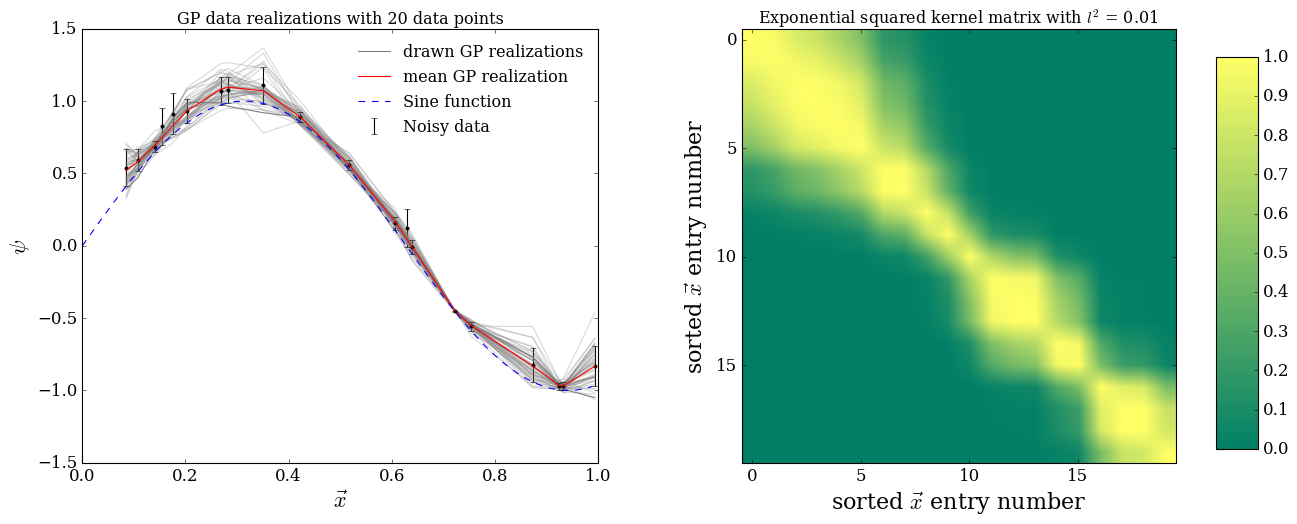
\includegraphics[width=0.9\linewidth]{expSq_kernel_demo_lsq_0pt01.png}
	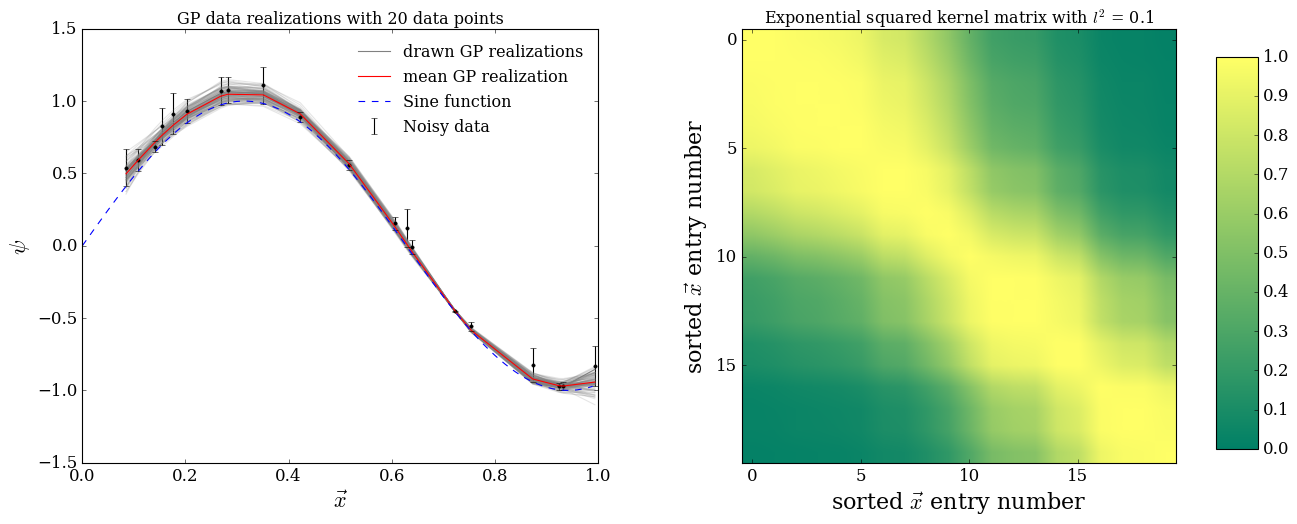
\includegraphics[width=0.9\linewidth]{expSq_kernel_demo_lsq_0pt1.png}
	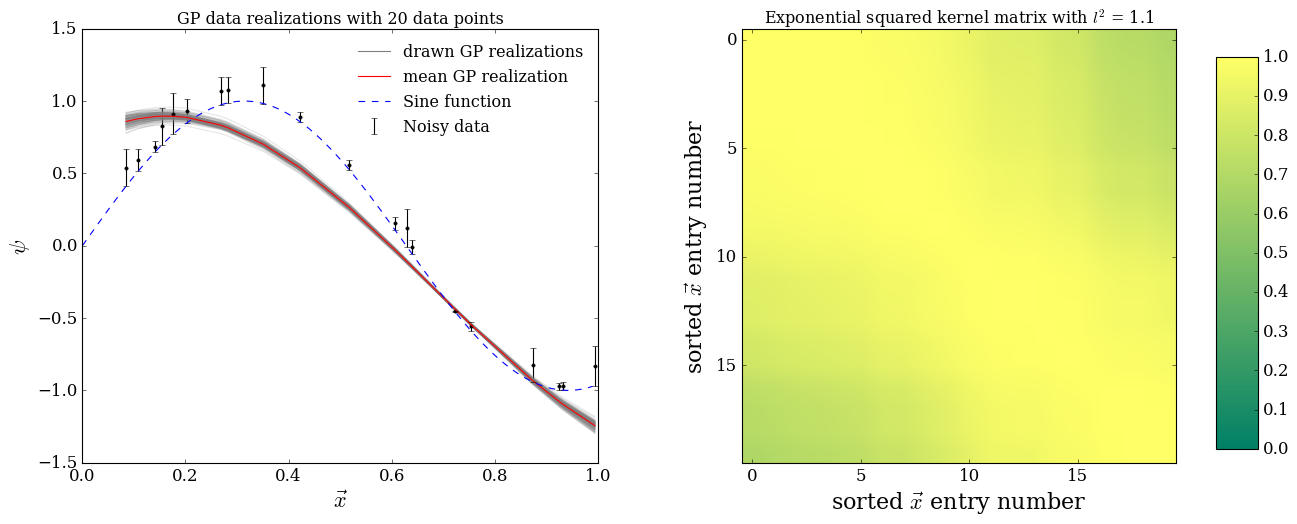
\includegraphics[width=0.9\linewidth]{expSq_kernel_demo_lsq_1pt1.png}
	\caption{
		We show GP models with different correlation lengths (left) and their
		corresponding kernel (right) on each row of this figure.
		Left: An example GP with a one-dimensional input vector $\xv_0$
		of length 20. The data points (($\psi_0, \xv_0$); black dots) 
		are generated from a sine function (blue dashed lines).  
		We added some Gaussian noise to the data points as indicated by the error bars. 
		The grey lines indicate the different realizations of
		the predictions given by the corresponding GP, while the red line indicates the
		mean realization.  
		Right: The corresponding exponential squared matrix that is used to model
		the GP on the left. 
		\label{fig:one_d_gaussian_process}}
\end{figure}


\subsubsection{An example: interpolating a set one-dimensional spatial inputs
with a GP}
\label{subsubsec:interpolation}
We illustrate the properties of an exponential squared covariance kernel $\kerngp$
by using the corresponding GP to interpolate a set of data $\psi_0$  
at a set of one-dimensional spatial location $\xv_0$, to a smoother version
$\psi$. 
This is visualized in Fig. \ref{fig:one_d_gaussian_process}.
% A set of one-dimensional spatial inputs $\xv_\mathds{1}$ can be thought of a set of 
% 2D coordinates along a line.  
% We show the data that we try to model in Fig. \ref{fig:one_d_gaussian_process}.
We compute 20 true data points $\psi_0$ (black points) from a sine function (blue dashed line) at
$\xv_0$.
Given $\xv_0$, we can then compute an exponential squared kernel matrix $\kerngp$ 
by assuming the values of the parameters of the covariance function
($\gpparams = [\lambda, l^2]$) to model the signal. 
We further add Gaussian noise ${\bf\epsilon}$ to the original data $\psi_0$ as
indicated by the individual error bar ($\sigma_i$). 
Since the noise contributions are drawn
from a Gaussian,
each of them adds variance to each data point, without adding covariances
between data points.
Mathematically, it means we can model the noise using a diagonal noise 
covariance kernel as part of a composite GP kernel. 
The resulting $\ngal \times \ngal$ composite kernel matrix for the observed data is:
\begin{equation}
	\Matrix{K}^\Matrix{C}_{m, n} = \lambda^{-1} \exp \left(-\frac{r_{m,n}^2}{2
	l^2}\right) + \sigma_n^2
	\delta_{m, n}
\end{equation}

In this interpolation problem, we want a way to find values of $\psi$ from our
model given the original data $\psi_0$ (black data points). We can do so by 
computing the conditional distribution of 
($\psi$, $\xv$) given ($\psi_0$, $\xv_0$). We also set $\xv = \xv_0$ to
interpolate at the original data position, but this is a choice, not a
restriction of the GP. It is possible to set $\xv$ to any location, but the 
interpolation (and predictions) works best when there are original data points
near the interpolated locations for training the GP model.

Recall the joint distribution of the data
described by a GP, by definition, is:
\begin{align}
	Pr(\psi, \psi_0 |\kerngp, \xv_0) = \mathcal{N}(0, \kerngp') &=  \mathcal{N}\left(\left[\begin{array}{c} 0 \\ 0 \end{array} \right], 
	\left(
	\begin{array}{cc}
		\kerngp(\xv, \xv) & \kerngp(\xv, \xv_0) \\
		\kerngp(\xv, \xv_0)^T & \kerngp(\xv_0, \xv_0) + \sigma_n^2 \mathds{1}
	\end{array}
	\right)
	\right)\\
&=  \mathcal{N}\left(\left[\begin{array}{c} 0 \\ 0 \end{array} \right], 
	\left(
	\begin{array}{cc}
		A & B \\
		B^T & C 
	\end{array}
	\right)
	\right),
\end{align}
where on the left hand side, $\kerngp$ represents the functional form of the
exponential squared kernel as a model.
The corresponding conditional distribution for modeling the interpolated values
$\psi$ is \citep{Rasmussen2006}:
\begin{align}
	Pr(\psi | \psi_0, \xv, \kerngp) &= \frac{Pr(\psi, \psi_0 |\kerngp,
	\xv)}{Pr(\psi_0 |\kerngp, \xv)} \label{eq:conditional_distribution0}\\
	&= \mathcal{N}(BC^{-1}\psi_0, A -
	BC^{-1}B^T).\label{eq:conditional_distribution}\\
	& \equiv \mathcal{N}(\mathbb{E}(\psi | \psi_0), \Cov(\psi | \psi_0))
\end{align}
Note that both the numerator and the denominator are Gaussians in eq.
\ref{eq:conditional_distribution0} for the final expression
\ref{eq:conditional_distribution} to be Gaussian. 
We can then draw different predictions of $\psi$ using:
\begin{equation}
	\psi \sim Pr(\psi | \psi_0, x, \kerngp).
\end{equation}

In eq. \ref{eq:conditional_distribution}, 
we can find the expected value of the conditional prediction of $\psi$ to be 
\begin{equation}
	\bar{\psi} = \mathbb{E}(\psi | \psi_0) = \kerngp(\xv, \xv_0)[\kerngp(\xv_0, \xv_0) +
	\sigma_n^2 \mathds{1}]^{-1}\psi_0, 
\end{equation}
where the multiplication of the different
components of the kernel $ [\kerngp(\xv_0, \xv_0) +
	\sigma_n^2 \mathds{1}]^{-1}$ to
the training points $\psi_0$ allows the kernel to weight $\psi_0$ to compute
the mean prediction $\bar{\psi}$. 
The weighting scheme is represented by the covariance matrix structure in the
right panels of Fig. \ref{fig:one_d_gaussian_process}.
The form of exponential squared function creates noticeable structures in the
kernel matrix, i.e. the yellow,
overlapping squares in the top right panel. 
Recall from eq. \ref{eqn:exp_sq_kernel} that 
the precision parameter $\lambda$ affects the 
amplitude of the correlations in the covariance matrix, while the correlation length (or
the characteristic length scale) $l^2$ 
determines how fast the correlations of  $\psi$ 
fall off across the spatial distance $r^2$. 
Such off-diagonal structures allow each element in the output vector $\psi$ to be weighted by
several neighboring spatial elements in $\psi_0$ as a form of smoothing.

As a result of the different correlation lengths for smoothing, 
the predictions fluctuate on specific spatial scales accordingly.
These realizations are represented by the gray lines in the left column of Fig.
\ref{fig:one_d_gaussian_process}. From the top row, we can see that 
the predictions that are drawn from a GP with a small $l^2$ 
fluctuate on a relatively small scale. Even the mean prediction (red line) over
different predicted realizations in the top
left panel is not completely smooth. When $l^2$ is increased as we show in the
middle and bottom left panels, we can notice that the predictions are
smoother, but the fit becomes worse as the $l^2$ value gets too big. 

To find the best GP parameter values, we can optimize 
the goodness of fit. A popular measure of the goodness of fit is
the log likelihood, which takes the form of:
\begin{equation}
	\log \mathcal{L} = \log(Pr({\bf d} | M))
\end{equation}
which denotes the PDF of obtaining the data vector ${\bf d}$ given the
statistical model $M$. 
In the case of the example in this section, the data vector is ${\bf d} =
\psi_0$. Our model is the GP, which is parametrized by mean
function (assumed to be zero) and the kernel matrix. 
Or in other words, our model is:
\begin{equation}
	\psi_0 \sim \mathcal{N}(0, \kerngp^\Matrix{C})
\end{equation}
So a consistent form of the log
likelihood is: \\
\begin{align}
	\log \mathcal{L} &= \log (Pr(\psi_0 | \kerngp^\Matrix{C}, \xv))\\
	&=  -\frac{1}{2}\psi_0^T {\kerngp^\Matrix{C}}^{-1}\psi_0
	- \frac{1}{2}\log|\kerngp^\Matrix{C}| - \frac{n}{2}\log(2\pi),
	\label{eq:log_marginal_likelihood0}
\end{align}
where the number of data point is $n=20$. Note that this expression gives a scalar output.
In fact, we can further interpret the composition of the log likelihood in 
eq. \ref{eq:log_marginal_likelihood0}. It
consists of a first term that describes the goodness of fit.
The second term penalizes complex model assumptions \citep{Rasmussen2006} 
as the determinant represents the volume of the hypersphere (e.g. product of
all the eigenvalues) spanned by the kernel matrix. 
The complexity penalization term can prevent the GP from overfitting the data.

% It is computed by 
% the conditional probability
% expression in \ref{eq:conditional_distribution}, but instead of
% drawing values from the expression, we compute a scalar value from the expression:
% \begin{equation}
% 	log Pr(\psi | \psi, \xv) = -\frac{1}{2}\psi_0^T\kerngp^{-1}\psi_0 -
% 	\frac{1}{2}\log|\kerngp'| - \frac{20}{2}\log(2 \pi)
% \end{equation}
% we call it as the log marginal 
% an optimal set of GP parameters $\gpparams^*$ are found by optimizing the log
% marginal (Gaussian) likelihood of a GP.
% \begin{equation}
% 	\log \mathcal{L} =  
% \end{equation}

Another noticeable property of a GP is the probabilistic nature of its predictions
(Fig. \ref{fig:one_d_gaussian_process}).
We can draw many realizations of the predictions to characterize our uncertainty. 
We can compute the 68\% credible levels
by using the minimum and maximum values of 68 out of 100 predictions at each
$\xv$ location.
In such a computation, the credible levels are wider for spatial regions 
with fewer and less certain data points. In the top left panel of Fig.
\ref{fig:one_d_gaussian_process}, we can see that the gray lines can have
larger discrepancies at data point locations $\xv$ with larger error bars, while they
have less discrepancies for data point locations with smaller error bars. 
% In fact, the possible interpolated values $\psi$ at a specific $\xv$ (along the vertical
% axis), under our GP model, also follow a Gaussian distribution \citep{Rasmussen2006}.  

% The probabilistic nature of the GP highlights the main differences of our
% approach vs past analysis approaches. While past analysis computes summary 
% statistics, such as the correlation-function to represent the  

\begin{table}%[htb]
% \small
\begin{center}
\caption{Parameters for our probabilistic model.}
\label{tab:sampling_parameters}
\begin{tabular}{cl}
\hline
Parameter & Description \\
\hline
$\kerngp$ & a general GP covariance kernel {\it matrix}, such as an exponential squared kernel \\
$\kerngp_{\rm GP}$  & the modified GP covariance kernel {\it matrix} that has incorporated
lensing physics\\
$\Matrix{S}$ or $\kerngp^\Matrix{C}$ & a composite GP kernel \\
${\bf d_{n}}$ & data vector (measured $e_{1,2}$ for each galaxy $n$)  \\
$\sigma_{{\rm ms}; n}$ & ellipticity measurement error for galaxy $n$ 
\\
$\xv$, $\yv$ & vector(s) of 2D spatial locations of galaxies \\
$\epsilon_n^{\rm int}$ & intrinsic galaxy ellipticity for galaxy $n$ \\
$\alpha\equiv\sigma_{e}^2$ & parameters of the distribution of galaxy parameters \\
W & window function for the survey footprint \\
$\lensparams$ & lensing shear and convergence ($\gamma_{1,2}, \kappa$) \\
$\gpparams$ & parameters of the GP kernel\\
% $\rho_{\rm GP}$ & correlation of the GP kernel (element of $\gpparams$) \\
$\lambda$ & precision of the GP kernel (element of $\gpparams$) \\
$l^2$ & squared GP correlation length (element of $\gpparams$) \\
% $\lambda_{\epsilon}$ & precision for the nugget term (element of $\gpparams$) \\
\hline
\end{tabular}
\end{center}
\end{table}
\subsection{Adapting the exponential squared kernel (matrix function) with lensing physics}
There are several families of commonly used covariance kernel.
The ones that are of the highest interest to cosmic shear modeling 
are {\it stationary kernels} that can capture 
the homogeneity and the isotropy of the data. This allows the predicted spatial fields
$\psi$ to have properties consistent with the large-scale matter distribution.
An example is the exponential squared matrix.
This kernel matrix $\kerngp(r^2)$ only depends on the
squared magnitude of distances between pairs of galaxy locations. 
This chosen form is, therefore, invariant
under translational and rotational transformations.
% The metric $\Matrix{D}$ is taken to be a diagonal matrix in this discussion but  
% can be generalized to account for anamorphic distortions due to the 
% flat sky approximation. Actual astronomical coordinates uses spherical
% coordinates instead of flat, 2D Euclidean coordinates. 

Additionally, the exponential squared kernel is infinitely differentiable. This
differentiable kernel choice allows us to derive an analytical expression to
relate the different lensing observables to enforce a consistent representation.  
With the use of the Born approximation\footnote{The deflection vector of the light ray by
	lensing is calculated by integrating the gravitational potential of the DM
	lens.  
	The Born approximation is the substitution of the integral by a 0-th order
	solution as a linear approximation. 
	This is explained in detail in Section 3.3 of \citealt{Kilbinger2015}.} in the linear regime, 
the scalar lensing potential $\psi$ is related to 
each of the lensing observables mentioned in chapter 1, e.g. 
$\lensparams \equiv [\kappa, \gamma_1, \gamma_2]$, via the following derivatives:
\begin{align}
\kappa &= \frac{1}{2}\left(\frac{\partial^2 \psi}{\partial x_1^2} +
\frac{\partial^2 \psi}{\partial x_2^2 }\right) 
= \frac{1}{2} (\psi_{,11} + \psi_{,22}),\\ 
\gamma_1 
&=\frac{1}{2}\left(\frac{\partial^2 \psi}{\partial x_1^2} - 
\frac{\partial^2 \psi}{\partial x_2^2}\right) 
= \frac{1}{2} (\psi_{,11} - \psi_{,22}), \\
\gamma_2 
&=\frac{1}{2}\left(\frac{\partial^2 \psi}{\partial x_1 \partial
x_2} + \frac{\partial^2 \psi}{\partial x_2 \partial x_1}\right)
= \frac{1}{2} (\psi_{,12} + \psi_{,21}),
\end{align}
where we have defined the shorthand for the derivatives of the two spatial dimensions with
subscripts $h,i,j,k = 1, 2$ after a comma.

We show how to derive one of the 6  covariance matrices that we can compute
from $\lensparams = [\kappa, \gamma_1, \gamma_2]$. The computation of the other
covariance kernels is completely analogous.
Since the covariance operator is linear, we can interchange the order of
operation between the covariance operator and the differentiation operators. 
\begin{align*}
&{\rm Cov}_{m,n} (\kappa(\vec{x}), \kappa(\vec{y}))  \\ 
&= \mathbb{E} \left[ 
	(\kappa - \mathbb{E}[\kappa])|_m 
( \kappa - \mathbb{E}[\kappa])|_n\right] 
\\
 &=\mathbb{E}\left[
\frac{1}{2} \left(\frac{\partial^2}{\partial y_1^2} + 
\frac{\partial^2}{\partial y_2^2}\right) 
 (\psi - \mathbb{E}\left[\psi\right])|_n \frac{1}{2}
\left(\frac{\partial^2}{\partial x_1^2} + \frac{\partial^2}{\partial x_2^2} \right)
(\psi - \mathbb{E}\left[\psi\right])|_m \right]
\\
&= \frac{1}{4}\left(
\frac{\partial^2}{\partial x_1^2} \frac{\partial^2}{\partial y_1^2} + 
\frac{\partial^2}{\partial x_1^2} \frac{\partial^2}{\partial y_2^2} +  
\frac{\partial^2}{\partial x_2^2} \frac{\partial^2}{\partial y_1^2} + 
\frac{\partial^2}{\partial x_2^2} \frac{\partial^2}{\partial y_2^2}  
\right) \kerngp_{mn},\\ 
\end{align*}
where $m, n = 1, 2, \cdots, \ngal$ represents the galaxy entry, and  
$\kerngp_{mn}$ denotes each element of the exponential squared kernel,
which is our chosen model for $\Cov(\psi, \psi)$.

The resulting 4th derivatives of the covariance
kernels $\kerngp_{\rm GP}$ have the following forms: 
\begin{align}
	\Cov (\kappa(\xv), \kappa(\yv))
&= \frac{1}{4}\left(
\kerngp_{,1111} + \kerngp_{,1122} + \kerngp_{,2211} + \kerngp_{,2222}
\right), \label{eq:kernel_derivatives1}\\
\Cov(\kappa(\xv), \gamma_1(\yv)) &= \frac{1}{4}\left(
\kerngp_{,1111} + \kerngp_{,2211} - \kerngp_{,1122} - \kerngp_{,2222}
\right), \\
\Cov(\kappa(\xv), \gamma_2(\yv)) &= \frac{1}{4}\left(
\kerngp_{,1112} + \kerngp_{,2212} + \kerngp_{,1121} + \kerngp_{,2221}
\right),\\
\Cov(\gamma_1(\xv), \gamma_1(\yv)) &= \frac{1}{4}\left(
\kerngp_{,1111} - \kerngp_{,1122} - \kerngp_{,2211} + \kerngp_{,2222}
\right), \\
\Cov(\gamma_1(\xv), \gamma_2(\yv)) &= \frac{1}{4}\left(
\kerngp_{,1112} + \kerngp_{,1121} - \kerngp_{,2212} - \kerngp_{,2221}
\right), \\
\Cov(\gamma_2(\xv), \gamma_2(\yv)) &= \frac{1}{4}\left(
\kerngp_{,1212} + \kerngp_{,1221} + \kerngp_{,2112} + \kerngp_{,2121}
\right), \label{eq:kernel_derivatives2}
\end{align}
where
\begin{equation}
	\kerngp_{,hijk} = \frac{\partial^4 \kerngp}{\partial x_h \partial x_i
	\partial y_j \partial y_k}.
	\label{eq:derivative_kernel}
\end{equation}

The differentiation by parts involves the differentiation of the distance matrix 
that we redefine here as:
\begin{equation}
	r_{m, n}^2 \equiv \sum_{i=1}^2 \sum_{j=1}^2 \Matrix{D}_{i, j}(\xv_{m, i} - \yv_{n, j}) (\xv_{m, i} - \yv_{n, j}), 
	\label{eq:distance}
\end{equation}
where $m, n = 1, 2, \cdots, \ngal$ represent the galaxy entries, the spatial
subscripts are $i, j = 1,
2$, and $\Matrix{D}$ is a diagonal Euclidean metric.
For each entry of the distance matrix, the differentiation takes the following
form:
\begin{equation}
	\frac{\partial r^2}{\partial \xv_i} = -\frac{\partial
	r^2}{\partial \yv_i} =
	2 \Matrix{D}_{i, i}(\xv - \yv)_i \equiv 2{\bf X}_i,
\end{equation}
where we define ${\bf X}_i$ as the spatial derivative of the distance matrix.

We show in Appendix \ref{app:GP_kernel_derivation} 
that each entry $\nu_{,hijk}$ of $\kerngp_{,hijk}$ is
related to each entry $\nu$ of the original exponential squared kernel
$\kerngp$ by:
\begin{equation}
\nu_{,x_h x_i y_j y_k} = (\beta^4 X_h X_i X_j X_k -
\beta^3 (X_h X_i \Matrix{D}_{jk} \delta_{jk} + 5~{\rm perm.}) + \beta^2
(\Matrix{D}_{hj} \Matrix{D}_{ik}\delta_{hj}\delta_{ik} + 2~{\rm perm.})) \nu
\label{eq:4thderivatives}
\end{equation}
with $\beta = l^{-2}$. There are 6 permutations (abbreviated as perm.) of the terms in
eq. \ref{eq:4thderivatives}
multiplied to $\beta^3$, as we can choose two pairs of indices from the $h,i,j,k$ 
when we differentiate the terms by parts, assuming that the order of each
pair of indices matters. 
Likewise, there are 3 possible permutations of
the terms the multiplied to $\beta^2$, as we can choose two pairs of indices from
$h, i, j, k$ where the order of the pairs does not matter.
The derivation of the relevant derivatives and terms are available 
in appendix \ref{app:GP_kernel_derivation} for completeness. 
Our implementation of the GP kernels in eq. \ref{eq:kernel_derivatives1} - 
\ref{eq:kernel_derivatives2} is also openly available at
\href{https://github.com/karenyyng/george}{https://github.com/karenyyng/george}.


\subsection{Making shear predictions (interpolation) with a GP}


\begin{figure}
	\centering
	\includegraphics[width=0.8\linewidth]{gp_cov_v2.png}
	\caption{An illustration of the GP covariance kernel matrix for the {\sc GalSim} data set.
		The same plot is also present in Schneider et al. (in prep.). We can see the various covariance
		and cross-covariance
		structures for the training data $\Upsilon = [\kappa, \gamma_1, \gamma_2]$
		and the interpolated data $\Upsilon' = [\kappa', \gamma_1', \gamma_2']$.
		% The spatial inputs in the example are sorted and taken from a line in the
		% 2D space $\xv$. 
		\label{fig:GP_kernel_vis}}
\end{figure}

Predictions of a GP are made using an appropriate conditional distribution as we have
shown in Section \ref{subsubsec:interpolation}. This time instead of a
one-dimensional set of inputs $\xv$, we have 2D coordinates $\xv$ and the
lensing observables are 2D spatial fields.
For predicting lensing observables, which are the convergence ($\kappa$) and
the two components of shear ($\gamma_{(1, 2)}$), we use a vector that is a concatenation of the
different lensing observables.  
We use $'$ to denote the quantities that we obtain
from the interpolation and quantities without prime represent the original data: 
\begin{equation}
[\lensparams', \lensparams]  = [\kappa', \gamma_1', \gamma_2', \kappa,
\gamma_1, \gamma_2] 
\end{equation}
The computation of the
conditional distribution mainly follows eq. \ref{eq:conditional_distribution}.
This time, only $\gamma_1$ and $\gamma_2$ are given in the data catalog from sky
surveys or simulations.  Values of
$\kappa, \kappa', \gamma_1', \gamma_2'$ are all inferred from the GP, we also
obtain a smoothed version of $\hat{\gamma_1}$ and $\hat{\gamma_2}$ from the GP.
In the presence of shape noise (intrinsic ellipticity) and measurement uncertainties, the actual 
expression of the conditional covariance kernel used for interpolation  
needs two additional diagonal white noise kernels.  
The partition of the kernel with the modified structure due to eq.
\ref{eq:kernel_derivatives1} to \ref{eq:kernel_derivatives2}
can be seen in Fig. \ref{fig:GP_kernel_vis}.

% Using the conditional distribution, 
% we can make predictions of $\kappa$ with data from the shear fields
% $\gamma_1, \gamma_2$. 
% Once we can find GP parameters $\gpparams^*$ that optimize the fit to
% the observed shear fields $\gamma_{(1, 2)}$ at $\xv$, we can compute $\kerngp_{(\kappa,
% \kappa)}$ and draw predictions of $\kappa$ from the conditional distribution. 
% Compared with an interpolation method, the mean predictions from a GP are
% often more well behaved and do not show drastic increase or decrease 
% in the tail regions where there is no data. 
% %
% Using a GP instead of a summary statistic also allows us to make predictions. 
% A prediction model can be any mathematical or numerical function that maps 
% the input data to the output appropriately. In the case of a GP, it relies on the covariance
% kernel structure to characterize this mapping.  
% 
\subsection{Obtaining physically interesting quantities from the modified GP}
\begin{figure}
	\centering
	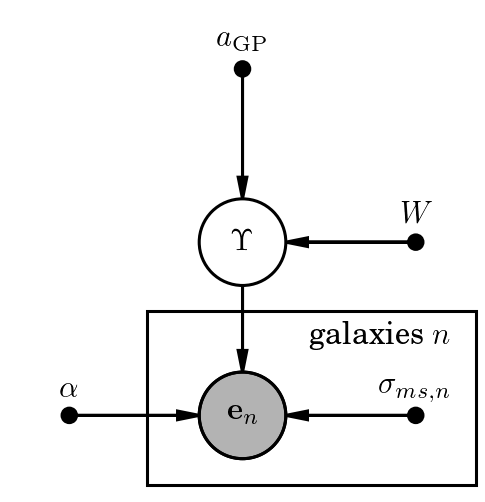
\includegraphics[width=0.4\linewidth]{shear_gp_pgm.png}
	\caption{A simplified probabilistic graphical model (PGM) for inferring
		the lensing observables $\Upsilon$ from survey or simulation data. The dots
		denote fixed parameters in the inference procedure. The empty circle denotes
		the latent variable, while the shaded circle denotes 
		the observed variable. The plate notation shows the observables that are
		implicitly summed over different galaxies during the computation of matrix-vector
		products in the log likelihood (eq. \ref{eq:log_marginal_likelihood}). The way that the observed
		ellipticity is connected to other branches hints that a joint analysis of
		the connected quantities will provide better predictive performance than if
		they were inferred separately. This figure is also present in Schneider et
		al. (in prep.).
		\label{fig:simplified_pgm}}
\end{figure}


By drawing realizations of the relevant GP, we can compute various 
physical quantities of interest. If the goal is to give the best prediction of a
mass map, it is possible to compute the mean realizations of the
convergence $\kappa$ from a conditional PDF
analogous to eq. \ref{eq:conditional_distribution}. 
We will show an example of this as a demonstration of
the consistency of our method with other known methods for making mass maps.
Or, if the shear statistics are of interest, the relevant 2PCF and the power
spectrum can be computed from the corresponding mean realization.

\subsubsection{Inferring the optimal GP parameters}
\label{subsubsection:optimize_GP_params}
Throughout the analyses present in this work, 
we make use of the weak shear approximation 
$g = \gamma / (1 - \kappa)  \approx \gamma$, so the observed ellipticity can be
modeled as: 
\begin{equation}
	\epsilon_{(1, 2)} = \epsilon_{\rm int} + g_{(1, 2)}, 
	\label{eq:weak_shear_approx}
\end{equation}
and we can express the contribution of the Gaussian shape noise $\epsilon_{\rm int}$
and the (Gaussian) measurement error $\sigma_{\rm ms}^2$
for each galaxy using a composite GP kernel:
\begin{equation}
	\mathsf{S} = \kerngp_{\rm GP} + \sigma_e^2 \mathds{1}  + \sigma_{\rm ms}^2
	\mathds{1}
	\equiv \kerngp_{\rm GP} + \mathsf{N}
	\label{eq:composite_kernel}
\end{equation}
where $\sigma_e^2$ is the variance of the shape noise, and $\sigma_{\rm ms}^2$
represents the measurement error. 
The log likelihood for our lensing analysis is: 
\begin{equation}
	\log p(\epsilon_{(1,2)} | \mathsf{S}, \xv) = \frac{-1}{2}\epsilon_{(1,2)}^T \mathsf{S}^{-1}
\epsilon_{(1, 2)}
- \frac{1}{2}\log|\mathsf{S}| - \frac{n}{2}\log(2\pi).
\label{eq:log_marginal_likelihood}
\end{equation}
% Note that for all other estimators for summarizing the lensing information, 
% one needs to separately assume a form of likelihood.  
We then use a numerical optimization routine such as gradient descent or 
Monte Carlo Markov Chains (MCMC)
to find the set of covariance kernel parameters $\gpparams^*$ that maximizes the
likelihood.
This allows us to infer a generalizable model for the observed shear. However,
this observed shear model still
contains contributions from both the shape noise and the measurement
uncertainties. 

\subsubsection{Reconstructing the signal using a Wiener filter}
From our model of the observed shear, 
we can reconstruct the noise-free shear signal using a Wiener filter (Wiener 1949). 
The Wiener filter is a linear operator $G$ that transforms the noisy
data to the signal:
\begin{equation}
	G\epsilon_{(1, 2)} = g_{(1, 2)}
\end{equation}
It works by minimizing the expected residual between the estimated signal and the true
signal. This technique has proven successful in the reconstruction of CMB signal
and power spectrum (\citealt{Elsner2013} and the references therein).
For signal and noise that are both Gaussian, the Wiener filter gives 
\begin{equation}
	p(\lensparams| \mathbf{d}, \gpparams, \sigma_{\rm ms}, \sigma_e) = \mathcal{N}(\mu_\lensparams,
	\mathsf{S}_\lensparams),
	\label{eq:Wiener_filter_posterior}
\end{equation}
with the data vector being $\mathbf{d} = \epsilon_{(1, 2)}$. We have assumed 
a GP model for the signal as a prior, and we plug in the
optimal GP parameters $\gpparams^*$ obtained from maximizing the log marginal
likelihood for the following quantities derived from the Wiener filter:
\begin{align}
\mu_\lensparams & = \kerngp_{\rm GP}(\kerngp_{\rm GP} + \mathsf{N})^{-1}
\epsilon_{(1, 2)}, \\
\mathsf{S}_\lensparams & = \kerngp_{\rm GP}(\kerngp_{\rm GP} +
\mathsf{N})^{-1}\mathsf{N}.
\end{align}
We use eq. \ref{eq:Wiener_filter_posterior}, which represents the posterior
of our Bayesian model to process two sets of
data for demonstration purposes. A representation of our map-making inference procedure can be seen in Fig. 
\ref{fig:simplified_pgm}. An alternative, but equivalent way of explaining this
model formulation can be found in more detail in Schneider et al. (in prep.).

\subsection{Validation data}
We checked our GP and probabilistic model in eq. \ref{eq:Wiener_filter_posterior}
against one set of synthetic data and one set of real data.
More details about the analysis and the related discussions are in Schneider et 
al. (in prep.).

\subsubsection{{\sc GalSim} data}
The first set of synthetic data that we analyzed was generated via the following procedure: 
We created an angular power spectrum of the convergence signal using {\sc
CHOMP}, a cosmology and halo model code\footnote{A fork of {\sc CHOMP} can be
found at \href{https://github.com/karenyyng/chomp}{https://github.com/karenyyng/chomp}
The original authors of CHOMP are Christopher Morrison, Ryan Scranton and Michael Schneider.
}. 
With a simulated convergence signal obeying this power spectrum, 
we generated lensed galaxy ellipticities using {\sc GalSim}, a modular galaxy image
simulation toolkit \citep{Rowe2015}.
In the process of generating the data, we specified 
the standard Lambda Cold-Dark Matter ($\Lambda$CDM) cosmology with $\Omega_m =
0.3$ and $\sigma_8 = 0.8$, using a narrowly peaked source redshift distribution
at around $z = 1$. As we can specify the intrinsic ellipticity variance
$\sigma_e^2$ from {\sc GalSim}, we made it deliberately small ($\sigma_e^2 =
0.00258$) to speed up our computationally expensive model. 
We also only made use of 1600 source galaxies, each centered on a pixel in a 
$40 \times 40$ grid. 
 
\subsubsection{The Deep Lens Survey (DLS) galaxy cluster Abell 781}
The second set of data was obtained from the DLS, an optical imaging survey 
designed for cosmic shear measurements.  
We illustrate that
our GP method can handle non-linear features, such as a galaxy clusters, and 
can compute a convergence map without problem. 
The data points
are centered on the galaxy cluster called Abell 781 in DLS field 2.
There are several previous lensing studies of this cluster, which has an estimated redshift
of $z \approx 0.296$ (\citealt{Wittman2014}, \citealt{Cook2012}, \citealt{Sehgal2008}). 
We selected source galaxies that have photometric redshift $z_b >
0.45$ and with small measurement uncertainties $\sigma_{\rm ms} < 0.1$. We also apply  
a R-band magnitude cut of $22 < R < 23$ and require the ellipticity for the
major (a) and minor axis (b) of the galaxies to satisfy $\sqrt{a^2 + b^2} > 0.8"$ 
to avoid selecting stars. We randomly selected 6000 galaxies that satisfy our
cuts for this analysis. From the selected galaxies, we evaluated the shape
root mean squared amplitude to be $\sim 0.21$, which we take to be the
intrinsic ellipticity scatter $\sigma_e$ in our inference.
Instead of fixing the value, the amplitude
$\sigma_e^2$ can also be inferred with a prior that brackets a reasonable range of
shape noise value.  
 
\section{Results}

\subsection{Validation using simulated data from {\sc GalSim}}
\begin{figure}[!ht]
	\centering
	\includegraphics[width=0.7\linewidth]{mass_map_comparison_galsim.png}
	\caption{A comparison of (right) the maps of the simulated data from {\sc GalSim}  and
	(left) the maps generated with the use of a GP prior. 
	This figure is a part of Schneider et al. (in prep.). \label{fig:Galsim_massmap}
}
\end{figure}
Fig. \ref{fig:Galsim_massmap} shows the mean posterior mass map obtained from
the {\sc GalSim} mock data. 
It shows features that are in general agreement with the true signal. 
It is noteworthy that the resolutions of the posterior maps are coarser ($24 \times 24$
spacing) than the input galaxy
spacing ($40 \times 40$). This reflects how the log likelihood
disfavors a sampling
scheme that is higher than the Nyquist frequency. The optimal smoothing length
($l^2 = 0.0123$) from the fitting routine of the log likelihood is also
larger than this Nyquist scale. As we speed up our code to handle a larger
volume and finer
resolution of input data, this limitation from the sampling scheme should
become negligible. We will discuss ways to speed up the computation to enable
the analysis of a denser catalog of data in Section
\ref{subsec:computational_performance}. 

From the averaged posterior map, we also computed the B-mode power spectrum.
The B-mode amplitudes are $< 2e^{-3}$ in the center of the field. 
The B-modes only have larger amplitudes $< 2e^{-2}$ at field boundaries.  
This is expected, as \cite{Bunn2003} have shown in a study of the CMB that 
the E and B modes can be mixed when the field of view is incomplete.
Although the B-mode amplitudes from our GP inference are small, 
improvements can be made 
if we understand what GP covariance kernel can represent the B-mode amplitudes to achieve complete E/B mode
separation.

\subsection{Mass mapping for Deep Lens Survey Abell 781}
\begin{figure}[h!]
	\centering
	\includegraphics[width=0.45\linewidth]{kappa_Abell781.png}
	\includegraphics[width=0.45\linewidth]{kappa_Abell781_WD.png}
	\caption{A comparison of mass maps for Abell 781 in the Deep Lens Survey (DLS) 
		\label{fig:Abell781_massmap}.  Left: The smoothed mass (convergence) map of Abell 781 from 
		our GP analysis of 6000 galaxies.
		Right: The higher resolution output generated with $\sim 50000$ galaxies using 
		algorithms from \cite{Wittman2014}. 
		There are five white crosses on each figure showing the locations of X-ray
		peak locations from \cite{Sehgal2008}. 
		% No clear mass has been associated
		% with the white cross second to the left. 
	These figures are from Schneider et al. (in prep.).
}
\end{figure}
We also see a general agreement of the features in the mass map of Abell 781
(Fig. \ref{fig:Abell781_massmap}) with previous studies of the same cluster 
\citep{Wittman2014}.  
We are restricted by the Nyquist frequency to give a coarser map as discussed
before.   
As the lensing signal from Abell 781 is high enough to beat the shape noise, 
we see an agreement of the inferred $\lensparams$ with \cite{Wittman2014}. 
We have not included enough galaxies to make a detailed comparison. 
This is also one of the reasons why  we
 have not inferred cosmological parameters using the
posterior maps of the DLS data.
% We have not inferred the existence of B-mode for the DLS data. 
% There are distortion from stacking exposures (e.g. visible chip gaps features) 
% and other observational limitations (e.g. masking of bright
% stars) that we have not corrected for. 


% Is a non-trivial optimization problem 

\section{Discussion}

\subsection{Relating the lensing observables to a cosmological model}
There is an ongoing effort to explore different ways to relate the posterior lensing signal 
to a cosmological model in Schneider et al. (in prep.). 
In this section, we outline some general ideas and concerns for such an effort. 
First, it is possible to use the GP as an intermediate representation, 
obtain estimators such as the 2PCF or the power spectrum from the GP predictions. 
Then use conventional techniques 
 to find the cosmological dependence from simulations.  
We can compute the shear-shear power spectrum from our mean posterior map of the shear with
corrected systematics. 
The resulting shear-shear power spectrum does not have variance contribution from the 
intrinsic ellipticites of the galaxies because the shape noise has been modeled
out by the Wiener filter. In conventional technique, the same marginalization
of the shape noise is done by averaging galaxies in the neighboring region.
The shear-shear power spectrum obtained in this manner can enable comparison to
cosmological simulations of the DM density field as outlined in previous studies (\citealt{Jee2013a},
\citealt{Semboloni2007}). Alternatively, if one wish to use the convergence
information instead, it is possible to the predicted values of the convergence
map to compute the convergence power spectrum. The convergence statistics may
be desirable because the computation of convergence quantities is simpler. The
convergence is a scalar field instead of a vector field like shear. 

Second, if we were to explore new ways to relate the GP outputs to cosmological constraints,  
it may be interesting to investigate the sensitivity of the GP parameters (and
the covariance kernel models) to cosmological parameters. 
Directly relating the GP parameters or the outputs of the GP to cosmology can
avoid unnecessary transformation and prevent the potential loss of cosmological 
information. 
We should note that the GP parameters may not be very sensitive to cosmological parameters
due to its flexibility to model a large variety of data. The sampling strategy of
the galaxy locations may also affect the sensitivity. Such a sensitivity test can be
done by repeating our {\sc GalSim} study using convergence power spectrum of different cosmology 
and different sampling. 
If we know the sensitivity of the GP parameters to cosmological parameters, 
we can design priors that broadly encompass current cosmological constraints 
to initialize and speed up the optimize of the GP likelihood. 

% Lastly, if the GP parameters are shown to be
% insensitive to cosmological parameters, it is also possible to use dimensionality
% techniques to find alternative features in the posterior map that can best determine the
% underlying cosmology. 
% \begin{figure}
% 	\centering
% 	\includegraphics[width=0.4\linewidth]{shear_general_pgm.png}
% 	\caption{A more general probabilistic graphical model (pgm) for inferring
% 		the lensing observables $\Upsilon$. The circle denotes
% 		latent variable, while the shaded circle denotes 
% 		the observed variable. The plate notation shows the galaxy entries to sum
% 		over.
% 		\label{fig:general_pgm}}
% \end{figure}

\subsection{The computational performance of the GP}
\label{subsec:computational_performance}
Another big consideration for any cosmic shear inference method is the 
computational performance.
Any computationally expensive algorithms for cosmic shear inference 
may become infeasible if it cannot analyze enough galaxies to 
capture the cosmological information at the different relevant length scales.
% As upcoming sky surveys such as the Large Synoptic Survey Telescope (LSST) will
% provide data from billions of source galaxies, 
% A computationally expensive method like the GP 
% may become infeasible if the algorithm cannot 
% analyze enough galaxies to capture features at different length scales. 
% For example, if a training data set happens to zoom in on 
% lensing data centered on a galaxy cluster with a field of view of
% several Mpc per side.
% The GP that is being trained using our derived kernel in eq.
% \ref{eq:derivative_kernel} on that set of data  
% will have GP parameters that every several Mpc along a dimension. 
% This is due to the homogeneity and isotropic requirement of our kernel. 
% This would contradict our knowledge that 
% galaxy clusters only appear at distances of tens of Mpc apart on average. 
%  
% We can visualize the predictions of the neighborhood of such a GP 
% to check for such anomaly in the model.  
% In our case, the computational cost is already an obstacle that keeps us from
% analyzing the entire DLS survey. 
% despite we have a parallelized implementation
% in a fast programming language.   
To achieve a high computational speed, we  
implemented the covariance kernels in eq. \ref{eq:kernel_derivatives1} to
\ref{eq:kernel_derivatives2}
in {\sc C++} along with a {\sc Python} wrapper. 
Although the operation of computing and assembling the
derivatives are $O(\ngal^2)$, the large number of addition and 
multiplication operations in eq. \ref{eq:kernel_derivatives1} to
\ref{eq:kernel_derivatives2} and \ref{eq:4thderivatives} can be slow.
Exploiting the symmetry of the covariance kernel can only provide 
a speed and memory saving of a factor of 2 for the matrix assembly step.

To make the computation run at a reasonable speed, 
I implemented the parallelized computation of each element of the kernel using 
the {\sc OpenMP} library. The slowest step of the entire computation, however, 
is the inversion of the
covariance kernel matrix for the evaluation of the marginal likelihood in eq.
\ref{eq:log_marginal_likelihood}, 
which is an $O(\ngal^3)$ operation. 
I made use of a multi-threaded version of the Cholesky decomposition via the {\sc Intel Math
Kernel Library} to invert the matrix. I achieved a $\sim10$ 
times speedup so the computation and the evaluation of the likelihood of each set of GP parameter
takes $\lesssim 3s$ for 1600 galaxies, which translates to 
the inversion of a 4200 $\times$ 4200 covariance matrix.
With the use of distributed computational resources, it is possible 
to probe the space of possible GP parameters by assigning each node to only
evaluate the log marginal likehood for one set of parameters. 
But the scalability of our method is limited by the available memory on each
computer node.

Currently, our method is not as computationally competitive as the 2PCF. 
The fastest implementation of 2PCF has a computational complexity of
$O(n_{\rm gal}\sqrt{n_{\rm gal}})$.
The 2PCF algorithm has also been demonstrated to scale almost linearly with
computational resources 
using a distributed and multi-threaded implementation \citep{Chhugani2012}. 

In terms of speed optimization for our method, rather than relying on 
a parallel computation of the kernel, there are several 
possible approximations that can provide huge speedup. 
Since there are many zero entries in the covariance kernel as shown in
Fig.\ref{fig:GP_kernel_vis}, it may be acceptable to put the kernel in a sparse
computational representation \citep{Snelson2007}. 
Thus, numerical libraries for sparse matrix 
operations (such as {\sc ScaLAPACK} or {\sc PLAPACK})
can provide speedup from looping over fewer data entries. 
An existing field of study that shows how the sparsity
approximation may affect the statistical inference is called covariance
tapering \citep{Kaufman2005}. 

On the other hand, there have been successes of further speedup for a GP than
pure sparsity approximations. This requires the introduction of  
 synthetic data sets called inducing points (\citealt{Snelson2006},
\citealt{Rasmussen2006}). Inducing points are latent variables that represent
hidden connections between the training data set and the test set. 
% It relies on fact that the majority of the information content 
%  may be embedded in certain direction (principal components) 
% in the high dimension of the data.
% The large number of data points specifies more about the initial conditions than the
% underlying cosmology.
With the help 
of inducing points,
the inversion of the covariance kernel can be sped up to
$O(M^2 n_{\rm gal})$ for
building the model and $O(M^2)$ for interpolating / predicting output functions
at a new number of inducing data locations M, with M $\ll n_{\rm gal}$ 
\citep{Snelson2006}. While the speedup from inducing point methods is
promising, careful studies need to be done to see how it affects the
inference of cosmological parameters. 
% We note that the vast amount of data
% points in other methods for cosmic shear information may contain more
% information about the initial condition than the cosmological parameters.
  
\subsection{Alternative kernel choice(s) for encoding the lensing physics}
Besides improving the computational performance, the model design of our GP can
also be refined.
Alternative choices for a covariance kernel for describing the lensing physics 
include the family of Mat\'{e}rn kernels:
\begin{equation}
	\kerngp(\xv, \xv') = \frac{1}{\Gamma(\nu)2^{\nu-1}}\left[
		\frac{\sqrt{2\nu}}{l}|\xv - \xv'|
	\right]^\nu K_\nu \left(\frac{\sqrt{2\nu}}{l}|\xv-\xv'|\right) 
\end{equation}
where $K_\nu$ is the modified Bessel function of the second kind, with an order
$\nu$, whereas $l$ is the characteristic length scale.
The smoothness of the data generated from a Mat\'{e}rn kernel is closely
related to the degree of freedom $\nu$ of the kernel. 
The higher degree of freedom it has, the smoother the spatial variations of the
drawn $\psi$ would be for the same characteristic length scale $l$.
Note that a Mat\'{e}rn kernel is also only differentiable to the $(\nu-1/2)$ order
\citep{Rasmussen2006}.
If we wish to relate our kernels to the lensing potential through the 4th
derivative, we can only use Mat\'{e}rn kernels with $\nu > 9/2$. 
When we take the limit of the degree of freedom of a Mat\'{e}rn kernel to infinity, 
we recover the exponential squared kernel. The inclusion of a Mat\'{e}rn kernel
in addition to an exponential squared kernel, therefore, can pick up features
that are less smooth. The use of an additional Mat\'{e}rn kernel may mitigate the
restrictions from Nyquist sampling, but this hypothesis should be verified with
numerical experiments. 

%  The manual differentiation of the analytical form of the kernels can be tedious,
% it may be desirable to generalize the derivation of derivatives. Technologies such
% as automatic differentiation can spreads factors of the derivatives over a tree
% structure to allow almost exact computation. 
 

\subsection{Modeling the systematics and noise via a composite kernel}
Besides kernels that describe homogeneous and isotropic data,
there are other types of periodic kernels that may be useful
in modeling systematics. 
Patterns such as masking or footprints of the telescope due to the
stacking of multiple exposures are obvious during the visualization of the
galaxy density for DLS. 
Previous studies of modeling the PSF
have made use of interpolation with polynomial splines of foreground stars 
for such a task (\citealt{Rowe2010},
\citealt{Jee2013a}).  Instead, a GP can be used to represent the PSF distortions
of foreground stars in a more generalizable way \citep{Berge2012} and be
applied as a prior. This allows a probabilistic connection of the 
PSF modeling to the rest of the
analysis. The successful examples of modeling systematics with a GP go beyond 
the aforementioned Wiener filter formulation \citep{Perez-Cruz2013}.

To pick up undetermined periodicity or patterns, 
we can use composite kernels with different covariance structures, 
which can be formed by the addition and/or multiplication of several kernels,
\begin{equation}
	\kerngp^{\Matrix{C}} = \sum_i \kerngp_i(\gpparams^i).
\end{equation}
By fitting for the best values for $\gpparams^i$, it is possible  
to pick up (sometimes non-obvious) patterns in the data. 
For the best illustration for pattern discovery with a GP, see
\cite{Duvenaud2013}.
It contains a famous GP example that makes use of a composite kernel for picking up both the 
short and long term periodic trends for carbon dioxide emission at Mauna Loa.
Additionally, it is physically interesting to examine whether the kernels that best 
fit systematics and masking can represent most of the B-mode components
from the data. 

\subsection{Comparison of the GP with existing methods for cosmic shear analysis}  
The GP is a powerful regression method for representing
cosmic shear information that can overcome some of the limitations of existing
methods. First, a major limitation of existing methods such as the 2PCF and the power
spectrum is the inability to capture non-linear information, 
such as galaxy groups, clusters, sheets and filaments.
There has been efforts to find statistics to represent such non-linearities.
Proposed estimators include the shear peak statistics 
\citep{Bard2014}, the aperture mass statistic, 
or the bispectrum that uses higher order statistic  
instead of 2-point statistics \citep{Kayo2012}.
% However, there is no consensus whether such higher order statistic can
% sufficiently capture the cosmological information encoded by non-linear structures (\citealt{Jasche2013},
% \citealt{Kayo2012}). 
As we have demonstrated using the data of Abell 781, 
there is no restriction from the
GP for modeling non-linear features such as a galaxy cluster. 
A GP can capture both the linear and non-linear cosmological information. 

Another major upcoming challenge for cosmic shear analysis is the proper
evaluation and handling of systematics. 
The Large Synoptic Survey Telescope (LSST) will
provide data of large enough volume such that the
constraints will be limited by systematics such as masking. 
Our inference method is one of the few available that allows interpolation 
to mitigate effects of masking as part of its formulation. Not only can it interpolate
missing shear information, we have shown that it can also predict convergence
information based on the shear estimates from galaxy shapes.
An alternative method that can also achieve interpolation 
is the Karhunen-Lo\'{e}ve (KL) transform proposed by \cite{VanderPlas2012a}. 
The Karhunen-Lo\'{e}ve transform infers and represents the shear field as 
orthogonal eigenmodes \citep{VanderPlas2012a}. 
Since the KL transform and GP decomposes the shear data according to features
at different spatial scales, both the KL transform and the GP have the potential 
for discovering patterns due to camera systematics.  

The way that GP represents the coupling of large and small scale fluctuation 
may 

Furthermore, both studies have the potential of capturing the non-linearity 
features:


% Most of the existing methods for represent lensing information are estimators.
% Estimators alone are insufficient to completely specify a model of the data.
% For example, the mean and the covariance are the two parameters of a Gaussian
% distribution. But the average value of the data drawn from a Gaussian, 
% which is an estimator of the mean, 
% is insufficient to summarize all the information for the underlying Gaussian 
% distribution. The summary statistics are the representation (realization) of the 
% data based on some model assumptions. For the 2PCF, the implicit model assumption is that any
% finite collections of $\lensparams$ have to follow a Gaussian distribution
% (this is a known property of the Gaussian random field). 
% The uncertainty information of the aforementioned estimators, 
% needs to be evaluated separately with a covariance matrix. The computation of
% the covariance matrix of 2PCF can be expensive as it involves the computation
% the uncertainties at pairs of the galaxies coordinates. 
% There is no direct comparison between such estimators to the GP, which is a model.
% It is more reasonable to compare the summary statistic of the GP, such as
% the mean prediction $\bar{\psi}$ to such estimators.  
% When maximizing the
% likelihood of a GP fit to the data, both the mean
% prediction and the covariance kernel of the predictions are simultaneously inferred.





% In terms of mass map making techniques 

% We have mentioned a number of summary statistic are existing methods for 
% representing one realization of the lensing information. 
% They alone cannot predict the values of the
% spatial field at other locations. They rely on other methods to account for
% masking or other systematics. The separate estimation of the systematics can 
% inadvertently introduce artifacts that can bias the cosmological parameter 
% estimates. 
% Furthermore, it is not easy to estimate the uncertainties for the summary statistics. 
% For the 2PCF, it relies on a 4 point estimate to characterize its covariance.

% While there are other models, such as the a Karhunen-Lo\'{e}ve analysis 
% in \citep{VanderPlas2012a}, it only fits to one set of data of the shear field. 
% It does not provide a probabilistic description of the shear. 
% 
% With the GP model, if there is a strong relationship between the cosmological
% model and the GP parameters,  

% - [ ] describe why the lensing observables shouldn't have a B mode 
% Since the lensing observables are the second derivatives of a scalar field,
% it is known that they should be curl free and only contain E-mode signal. 

% It is well known that gravitational lensing, as presented in chapter 1,
% only induces a curl-free (E-mode) shear signal. However, the computation of 
% summary statistics at certain length scale can induce a B-mode (with non-zero
% curl) signal. 

%  \begin{align}
% 	\kappa^E & = \kappa\\
% 	\kappa^B & = 0 \\
% 	\gamma^E &= \left[\frac{1}{2} (\psi^E_{,11} - \psi^E_{,22}) -
% 	\psi^B_{,12}\right]\\
% 	\gamma^B &= \left[\psi^E_{,12} + \frac{1}{2} (\psi^B_{,11} - \psi^B_{,22})\right]
% \end{align}
% Can handle sharp boundaries from stacking images 
% cite Jee2013a  
% cite Rowe2010 paper for interpolating star fields for 
% PSF ellipticity corrections 



\section{Conclusion}
We have derived and implemented a fully probabilistic method for 
representing the lensing observables. 
Our modified GP possesses the following properties that may be desirable
for lensing analysis: \\ 
1) We have enforced a consistent probabilistic representation of the lensing 
observables. It is possible to predict a covergence map from the GP using
the same GP parameters of the shear map and vice versa.\\ 
2) The GP can specify the joint PDF of both the signal and the noise. 
This allows a natural way of propagating and correcting for error.\\
3) The GP provides a natural mechanism for interpolating  
and predicting values for unobserved regions. Using a conditional distribution, 
we can predict and interpolate new values based on the  information carried by
the covariance kernel(s).
\\ 
4) By analyzing two sets of data, 
we have demonstrated reasonable agreement between our method and both the true
simulated signal or with past analysis techniques.  \\
5) In our example from {\sc GalSim}, we have shown that the GP does not
introduce B-mode contamination. \\
6) We have shown that the GP can model non-linear gravitational structures such 
as a galaxy cluster. \\ 
7) In future studies, it may be possible to identify a GP kernel that is the most 
sensitive to the changes in cosmological parameters. Similarly, it may be
possible to identify kernels for capturing the noise and systematics components 
that are manifested as B-mode observables.

Due to the high computational complexity $O(\ngal^3)$ of the current
implementation of our GP method,  
the potential of using a GP for the inference of cosmological
constraints remains to be proven.
If those challenges can be solved with some of our
suggestions, the GP model can be 
extended to provide a joint analysis of cosmic shear along with 
the systematics and noise. 





% Requires the understanding of the underlying physical observable, how the statistical
% approach can carry the information and how to actual execute the computation in
% a tractable way.


\section{Acknowledgement}
We thank Chris Paciorek for discussion about the statistical
framework for performing shear inference and the
use of Gaussian Processes.
This research
used the resources of the National Energy Research Scientific 
Computing Center (NERSC), a DOE Office of Science
User Facility supported by 
of the U.S. Department of Energy under Contract No.
DE-AC02-05CH11231.
 This work uses a modified version
of the public code for GP inference {\sc George} available at \href{https://
github.com/karenyyng/george}{https://
github.com/karenyyng/george}, which was forked from \\
\href{https://github.com/dfm/george}{https://github.com/dfm/george}.



